\chapter{Аналитический раздел}
В этом разделе будут рассмотрены основные алгоритмы поиска редакционного расстояния, а также варианты их реализаций.

\section{Расстояние Левенштейна}
Расстояние Левенштейна\cite{Levenshtein} - минимально необходимое количество редакторских операций (удаление, вставка, замена) для преобразования одной строки в другую.
Всего используется четыре возможные редакторские операции:
\begin{itemize}
    \item I (англ. insert) - вставить;
    \item D (англ. delete) - удалить;
    \item R (англ. replace) - заменить;
    \item M (англ. match) - совпадение.
\end{itemize}
Операции I, D и R имеет цену, равную 1, а M - 0, так как в случае совпадения букв никаких действий не должно быть произведено.

\section{Обобщённый алгоритм для определения расстояния Левенштейна}
Пусть $s_{1}$ и $s_{2}$ - строки, для которых мы должны определить расстояние Левенштейна.
Индикаторная функция $m$ для двух символов $a$ и $b$ рассчитывается по формуле \ref{eq:M}:
\begin{equation}
	\label{eq:M}
	m(a, b) = 
 	\begin{cases}
 		1 &\text{, если a = b}\\
   		0 &\text{иначе}
 	\end{cases}
\end{equation}

Для строк $s_1$ и $s_2$ ставится в соответствие функция $D$, которая принимает на вход два индекса и рассчитывает ответ по формуле \ref{eq:D}:
\begin{equation}
	\label{eq:D}
	D(i, j) = \begin{cases}
		0 &\text{i = 0, j = 0}\\
		i &\text{j = 0, i > 0}\\
		j &\text{i = 0, j > 0}\\
		\min \lbrace \\
			\qquad D(i, j-1) + 1\\
			\qquad D(i-1, j) + 1 &\text{i > 0, j > 0}\\
			\qquad D(i-1, j-1) + m(a[i], b[j])
		\rbrace
	\end{cases},
\end{equation}

Функция $D$ составлена из следующих соображений:
\begin{itemize}
	\item для перевода из пустой строки в пустую требуется ноль операций;
	\item для перевода из пустой строки в строку $a$ требуется $|a|$ операций;
	\item для перевода из строки $a$ в пустую требуется $|a|$ операций.
\end{itemize}

Для перевода из строки $a$ в строку $b$ требуется выполнить последовательно некоторое количество операций (удаление, вставка, замена) в некоторой последовательности. Последовательность проведения любых двух операций можно поменять, порядок проведения операций не имеет никакого значения. Полагая, что $a', b'$  — строки $a$ и $b$ без последнего символа соответственно, цена преобразования из строки $a$ в строку $b$ может быть выражена как:
	\begin{itemize}
		\item сумма цены преобразования строки $a$ в $b$ и цены проведения операции удаления, которая необходима для преобразования $a'$ в $a$;
		\item сумма цены преобразования строки $a$ в $b$  и цены проведения операции вставки, которая необходима для преобразования $b'$ в $b$;
		\item сумма цены преобразования из $a'$ в $b'$ и операции замены, предполагая, что $a$ и $b$ оканчиваются разные символы;
		\item цена преобразования из $a'$ в $b'$, предполагая, что $a$ и $b$ оканчиваются на один и тот же символ.
	\end{itemize}

Минимальной ценой преобразования будет минимальное значение приведенных вариантов.

Пусть \begin{math} N_1 = |s_1|, N_2 = |s_2| \end{math}, тогда расстояние между строками $s_{1}$ и $s_{2}$ можно подсчитать по формуле \ref{eq:rho}:

\begin{equation}
	\label{eq:rho}
	\rho_л(S_1, S_2) = D(N_1, N_2)
\end{equation}

Все алгоритмы подсчёта расстояния Левенштейна работают именно с этим алгоритмом, лишь используя разные типы данных.

\section{Рекурсивный алгоритм для определения расстояния Левенштейна}
Рекурсивный вариант напрямую реализует формулу \ref{eq:D}, вызывая функцию $D$ для величин, равных длине каждой из строк. 
Стоит отметить, что порядок рекурсивного вызова подпрограмм не имеет значения. 
База рекурсии - первые три условия, поэтому гарантировано, что на выходе будет однозначный ответ.
Из недостатков сразу можно отметить, что одно и то же значение будет подсчитано несколько раз, поэтому будет происходить большое количество повторных операций.

\section{Рекурсивный алгоритм для определения расстояния Левенштейна с использованием матрицы}
В качестве оптимизации прошлого алгоритма можно подсчитанные значения сохранять в матрицу, в которой строкам i и j будет соответствовать значение функции $D(i, j)$. Каждый раз при подсчёте $D$ программа будет проверять, было ли уже подсчитано значение для заданных аргументов - и использует при существовании уже готовый вариант.

\section{Итеративный алгоритм для определения расстояния Левенштейна с использованием матрицы}
Можно обойтись и без рекурсивных вызовов подпрограмм, сразу заполняя в матрицу значения функции $D(i, j)$.

Сразу можно заполнить первую строку матрицы и первый столбец матрицы: для них условие тривиально. 
После этого процесс продолжается вдоль каждой строки до того момента, как подсчитано значение для последней клетки - в ней и будет содержаться ответ.
На рисунке \ref{fig:my_label} представлена работа итеративного алгоритма.


\begin{figure}[h]
    \begin{center}
        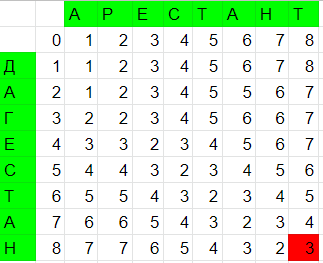
\includegraphics[width=13cm, height=12cm]{inc/МатрЛевен.png}
    \end{center}
    \caption{Иллюстрация работы матричного алгоритма нахождения расстояния Левенштейна}
    \label{fig:my_label}
\end{figure}

\section{Оптимизированный итерационный алгоритм для определения расстояния Левенштейна с хранением двух строк}
В вычислениях используются только две строки матрицы, поэтому можно не хранить всю матрицу, а лишь прошлую строку и ту, для которой производятся вычисления. Это позволяет существенно оптимизировать затраты по памяти.

\section{Расстояние Дамерау-Левенштейна}
Зачастую пользователь допускает опечатку, перепутав местами соседние буквы. Обычное расстояние Левенштейна для таких строк равно двум, поэтому для оптимизации таких ситуации было создано расстояние Дамерау-Левенштейна\cite{ifmo}.

К существующим операциям добавляется ещё одна - X (англ. Exchange). Штраф за неё также составляет один балл. Тогда функция $D$ вычисляется по формуле \ref{eq:d}:
\begin{equation}
	\label{eq:d}
	d_{a,b}(i, j) = \begin{cases}
		\max(i, j), &\text{если }\min(i, j) = 0,\\
		\min \lbrace \\
			\qquad d_{a,b}(i, j-1) + 1,\\
			\qquad d_{a,b}(i-1, j) + 1, &\text{иначе}\\
			\qquad d_{a,b}(i-1, j-1) + m(a[i], b[j]),\\
			\qquad \left[ \begin{array}{cc}d_{a,b}(i-2, j-2) + 1, &\text{если }i,j > 1;\\
			\qquad &\text{}a[i] = b[j-1]; \\
			\qquad &\text{}b[j] = a[i-1]\\
			\qquad \infty, & \text{иначе}\end{array}\right.\\
		\rbrace
		\end{cases},
\end{equation}

Для вычисления расстояния Дамерау-Левенштейна можно применять и итеративный, и рекурсивный метод вычислений. В работе будет использоваться рекурсивный вариант с заполнением матрицы для уже подсчитанных значений.

\section{Вывод}
В этом разделе был рассмотрен обобщённый алгоритм для нахождения расстояния Левенштейна, а также его три реализации:
рекурсионная, рекурсионная с матрицей и итеративная. 
Также было рассмотрено расстояние Дамерау-Левенштейна.
Для выполнения поставленных задач будет реализовано четыре алгоритма:
\begin{itemize}
	\item оптимизированный итеративный алгоритм поиска расстояния Левенштейна;
	\item рекурсионный алгоритм поиска расстояния Левештейна;
	\item рекурсионный алгоритм поиска расстояния Левенштейна с хранением матрицы;
	\item рекурсионный алгоритм поиска расстояния Дамерау-Левенштейна с хранением матрицы.
\end{itemize}